%----------------------------------------------------------------
%
%  File    :  thesis-style.tex
%
%  Author  :  Keith Andrews, IICM, TU Graz, Austria
%
%  Created :  27 May 93
%
%  Changed :  19 Feb 2004
%
% styling and technical implementation adopted 2011 by Karl Voit
%----------------------------------------------------------------

					\section{Analyse von Gleichstromnetzwerke}
					\label{chap:Style}


					\subsection{Strom, Spannung und Widerstand}


					Zwischen zwei unterschiedlich geladenen Punkten entsteht ein \textbf{elektrisches Feld}. Geladene Teilchen spüren eine Kraft in Richtung dieser Feldlinien. \\

					\begin{center}
						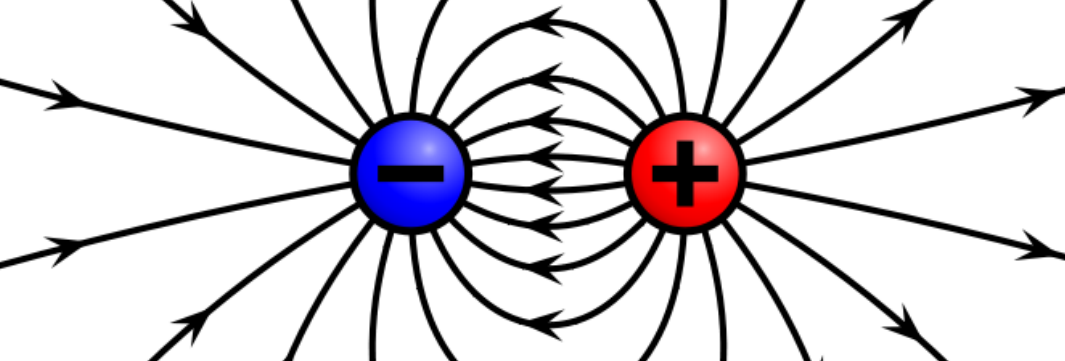
\includegraphics[scale=0.2]{img/e-feld.png}
					\end{center}


					\definition{Spannung}

           \beginip
						Wir definieren die Spannung zwischen zwei Punkten als das Wegintegral über das elektrische Feld: \\
						\formulaBegin
						$ U_{AB} :=  \int_A^B \vec{E} \cdot d\vec{s} $
						{[U]} = Volt {[V]}
						\formulaEnd
          \iend

					\subparagraph{Bemerkung}

					\begin{addmargin}[1em]{0cm}
						\vspace{-2mm}
						Da die Beziehung $\vec{F} =  q \cdot \vec{E} $ gilt und die Arbeit als $ W_{AB} = \int_A^B \vec{F} \cdot d\vec{s}$ definiert ist, können wir die Spannung zwischen zwei Punkten als \textbf{Maß der benötigten Arbeit} um ein Ladungsträger von A nach B zu bringen betrachten.
					\end{addmargin}


					\definition{Strom}

          \beginip
          Als Strom bezeichnen wir die Menge von Ladungen welche in einer gewissen Zeit durch eine Fläche fließen. \\

						\formulaBegin
						$ I := \frac{\texttt{\#}Ladung}{Zeit} = \frac{dQ}{dt}$
						{[I]} = \textbf{A}, Ampère
						\formulaEnd
					\iend

\newpage
			    \definition{Widerstand und Leitwert}

          \beginip
					Der \textbf{Widerstand} bestimmt, wieviel Strom fließen kann, wenn eine bestimmte Spannung angelegt wird. \\
					Ist der Wert des Widerstandes unabhängig vom Strom, so bezeichnen wir ihn als ohmschen Widerstand.
					\begin{center}
						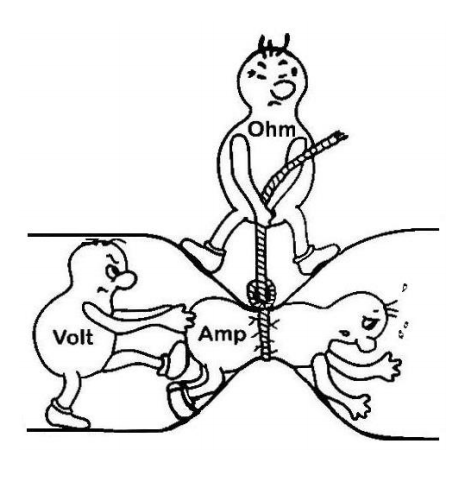
\includegraphics[scale=0.25]{img/widerstand.png}
					\end{center}
					\formulaBegin
					$ R :=  \frac{U}{I} =  \rho  \frac{l}{A},   {[R]} = \Omega, Ohm $
					\formulaEnd
					Als \textbf{Leitwert} bezeichnen wir die Inverse des Widerstandes. Er gibt an, wie groß die Spannung ist, wenn ein gewisser Strom fließt. \\
					\formulaBegin
					$ Y = \frac{1}{R} = \frac{A}{\rho \cdot l} $
					\formulaEnd
					\iend

					Da das elektrische Feld wirbelfrei ist, erhalten wir unabhängig vom Weg den gleichen Wert für die Spannung $ U_{AB} $ \\
					Dies bedeutet jedoch auch, dass wir für einen geschlossenen Weg die Spannung $0V$ erhalten müssen, da für jede geschlossene Kurve $\gamma$ gilt:
					\begin{center}
						\vspace{-2mm}

						$\displaystyle \int_{\gamma} \vec{E} \cdot d\vec{s} = \int_{\gamma_0}^{\gamma_1} \vec{E} \cdot d\vec{s} + \int_{\gamma_1}^{\gamma_0} \vec{E} \cdot d\vec{s} = U_{01} + U_{10} = 0$
					\end{center}
					Mit dieser Erkenntnis können wir die Maschenregel definieren:

					\definition{Maschenregel}
					\beginip
					Die Summe aller Spannungen in einer Masche ergibt $0$ \\
					\formulaBegin
					$\displaystyle \sum_{k=1}^n U_k = 0$
					\formulaEnd

					\iend

					\begin{minipage}{0.6\textwidth}
						\begin{flushright}
						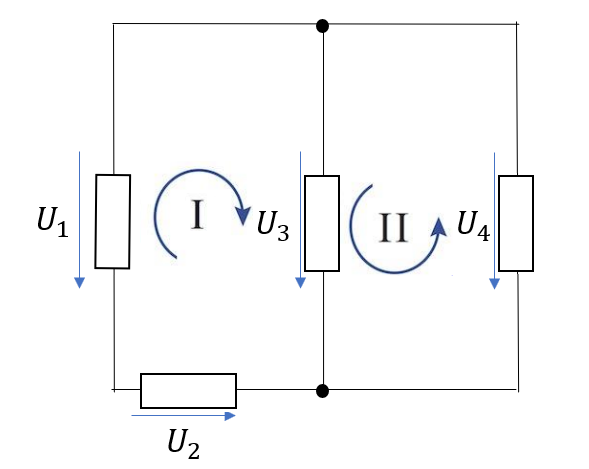
\includegraphics[scale=0.45]{img/maschenregel-2.png}
					\end{flushright}
					\end{minipage}
					\begin{minipage}{0.4\textwidth}
						\textbf{Maschenregel} \\ \\
						I: $\displaystyle (- U_1) + U_3 + (-U_2)  = 0$ \\
						II: $\displaystyle U_3 + (- U_4) = 0 $ \\
						% \vspace{1.5cm}
					\end{minipage}

					Analog können wir mithilfe der Ladungserhaltung argumentieren, dass sämtliche Ladungen, welche in ein Gebiet hineinfließen, auch wieder aus diesem hinausließen müssen.

					\definition{Knotenregel}
					\beginip
					Die Summe aller Ströme die in einen Knoten hinein/hinausfließen muss $0$ ergeben. \\
					\formulaBegin
					$\displaystyle\sum_{i=0}^n I_n = 0 $
					\formulaEnd
          \iend

					\textbf{Wichtig} Die Knotenregel kann auch auf ein Gebiet von Knoten angewandt werden. \\


					\begin{minipage}{0.6\textwidth}
					\begin{flushright}
							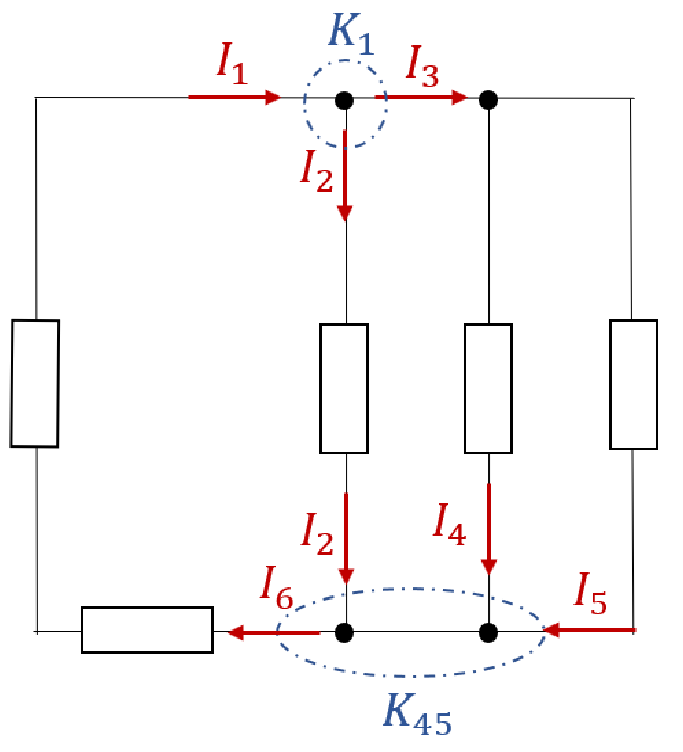
\includegraphics[scale=0.4]{img/knotengl.png}
						\end{flushright}
					\end{minipage}
					\begin{minipage}{0.4\textwidth}

						\textbf{Knotengleichungen} \\ \\
						$\displaystyle K_1$: $ I_1 - I_2 - I_3 = 0 $ \\
						$\displaystyle K_{45}$: $ I_2 + I_4 + I_5 - I_6 = 0 $ \\
					\end{minipage}


\newpage

					\subsection{Grundlegende Netzwerkumformungen}
					Wir interessieren uns nun dafür, wie sich Widerstände verhalten, wenn wir sie seriell/parallel verknüpfen.
					\definition{Serienschaltung}
					\beginip
					Werden mehrere Widerstände seriell miteinander verbunden, so addieren sich die Widerstandswerte \\
					\formulaBegin
					$\displaystyle R_{serie} = \sum_{i=0}^n R_i $
					\formulaEnd
					\iend

		        \vspace{1em}

					\textbf{Begründung} \\
					Mehrere Widerstände in Serie können als ein langer Widerstand mit konstanter Fläche angesehen werden. Da die Längenabhängigkeit des Widerstandes im Zähler steht, addieren sich die Werte. \\
					$\displaystyle R_s = \rho \cdot \frac{l_1+l_2}{A} = \rho \cdot \frac{l_1}{A}  + \rho \cdot \frac{l_2}{A}  = R_1 + R_2 $
					\fix
					\begin{center}
						\ibox{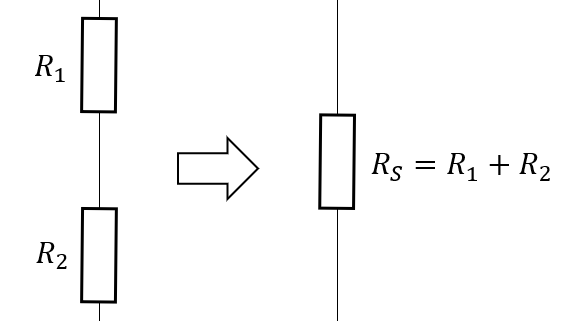
\includegraphics[scale=0.3]{img/serienschaltung.png}}
					\end{center}
\fix


					\definition{Parallelschaltung}

					\beginip
					Werden mehrere Widerstände parallel miteinander verbunden, so addieren sich die Leitwerte \\
					\formulaBegin
					$\displaystyle Y_{parallel} = \sum_{i=0}^n Y_i \Bigg\rvert$
					$\displaystyle R_{parallel} = \left(\sum_{i=0}^n \frac{1}{R_i}\right)^{-1}$
					\formulaEnd
					\iend

          \vspace{1em}

          \textbf{Begründung} \\
					Mehrere Widerstände parallel können als ein Widerstand mit größerer Fläche und konstanter Länge angesehen werden. Da die Flächenabhängigkeit des Widerstandes im Nenner steht, addieren sich die Leitwerte. \\
						$\displaystyle Y_p = \frac{1}{\rho} \cdot \frac{A_1 + A_2}{l} = \frac{1}{\rho} \cdot \frac{A_1}{l}  + \frac{1}{\rho} \cdot \frac{A_2}{l}  = Y_1 + Y_2 $


					\begin{center}
						\ibox{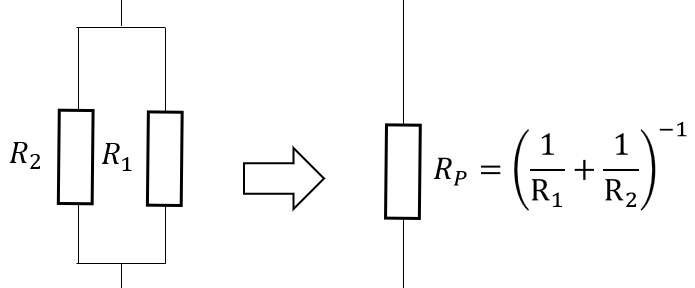
\includegraphics[scale=0.3]{img/parallel.png}}
					\end{center}


					\definition{Spannungsteiler}
					\beginip
					Die Spannungsteilerregel gibt an, wie sich eine Spannung über verschiedene Widerstände aufteilt, wenn diese in \textbf{Serie} geschaltet sind. \\
						\formulaBegin
						$\displaystyle U_{R_x} = U_{ges} \cdot \frac{R_X}{\sum R_i} $
						\formulaEnd

						\begin{center}
							\ibox{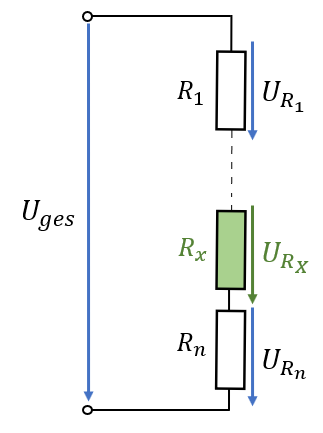
\includegraphics[scale=0.4]{img/spannungsteiler.png}}
						\end{center}
					\iend


					\textbf{Begründung} \\
						Gemäss $\displaystyle U = R \cdot I $ und der Serienschaltung ist der Strom durch alle Widerstände gegeben als $\displaystyle I = \frac{U_{ges}}{\sum R_i} $ \\
						Nun müssen wir nur noch den Strom mit dem gesuchten Widerstand multiplizieren um die Spannung zu erhalten: $\displaystyle U_{R_X} = R_X \cdot I = R_X \frac{U_{ges}}{\sum R_i} $

\fix
					\definition{Stromteiler}
					\beginip
						Die Stromteilerregel gibt uns an, wie sich die Ströme in einem Knoten aufteilen, wenn die Widerstände \textbf{parallel} geschaltet sind.
						\fspace
						\formulaBegin
						$\displaystyle I_x = I_{in} \cdot \frac{(R_1 || ... || R_n)} {R_x} $
						\formulaEnd
\fix
						\begin{center}
							\ibox{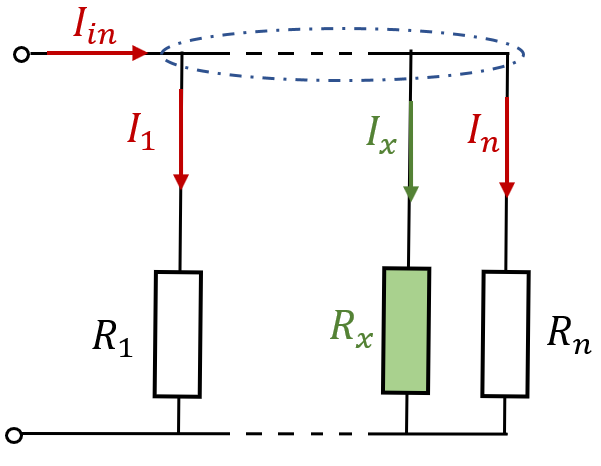
\includegraphics[scale=0.3]{img/stromteiler.png}}
						\end{center}
						\fix
						\textbf{Spezialfall} 2 Widerstände \\
						Falls der Stromteiler nur mit zwei Widerständen angewendet wird, vereinfacht sich die Formel:
						\fspace
						\formulaBegin
						$\displaystyle I_x = I_{in} \cdot \frac{R_y}{R_x + R_y} $
						\formulaEnd
						Der Widerstand, dessen Strom uns \textbf{nicht} interessiert, steht hierbei im Zähler!
					\iend

					\subsubsection{Grundregeln bei Netzwerkumformungen}
\fix \fix
					\important{Regel 1}{Expandieren von Knoten}
					\beginip
					 	Knoten können aufgeteilt und mit Verbindungslinien verbunden werden\\
						\begin{center}
						\ibox{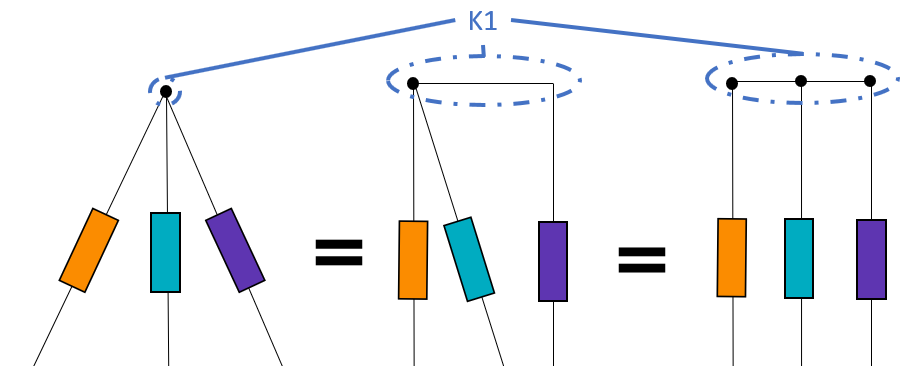
\includegraphics[scale=0.25]{img/knotenexp.png}}
						\end{center}
					\iend

					\fix
\fix \fix
					\important{Regel 2}{Verschieben von Elementen}
					\beginip
						Elemente können entlang von \textbf{Verbindungslinien ohne Widerständen} verschoben werden\\
						\begin{center}
							\fix \fix \fix
						\ibox{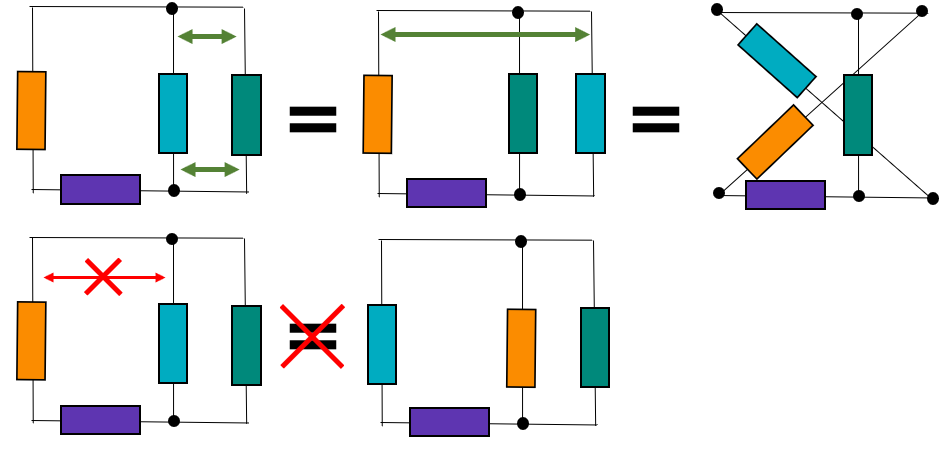
\includegraphics[scale=0.3]{img/verschieben.png}}
						\end{center}
					\iend
\fix \fix
					\important{Regel 3}{Vertauschen von Elementen in Serie}
					\beginip
						Elemente, die \textbf{in Serie} geschaltet sind, können vertauscht werden
						\begin{center}
							\fix
						\ibox{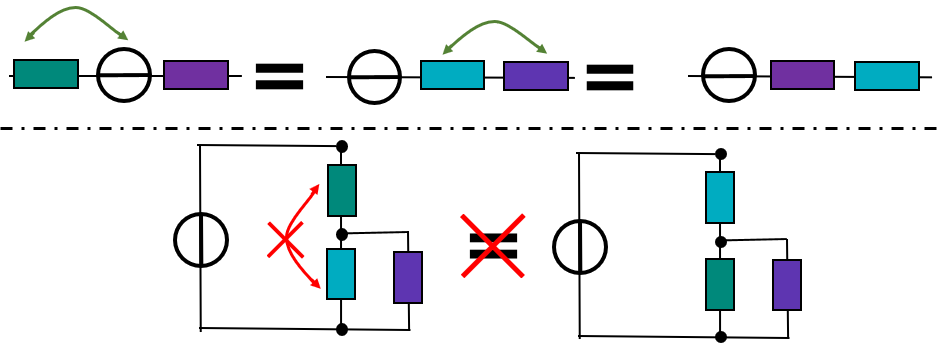
\includegraphics[scale=0.3]{img/vertausch-serie.png}}
						\end{center}
					\iend
\fix \fix
					\important{Regel 4}{Vertauschen von parallel geschalteten Elementen}
					\beginip
						Elemente die \textbf{parallel} geschaltet sind, können vertauscht werden
						\begin{center}
							\fix
						\ibox{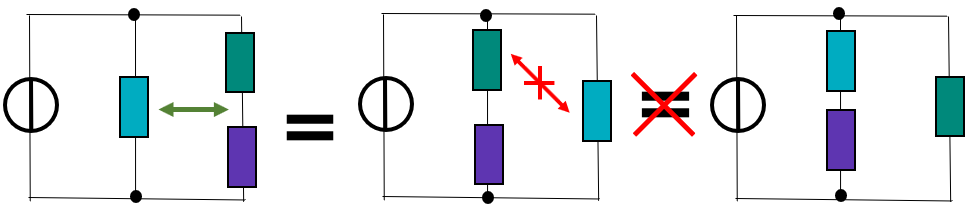
\includegraphics[scale=0.3]{img/vertausch-parallel.png}}
						\end{center}
					\iend
\fix \fix
					\important{Regel 5}{Knoten kontrahieren}
					\beginip
						(Analog zu 1) Knoten können zusammengezogen werden, sofern sie nicht durch einen Widerstand verbunden sind.
						\begin{center}

						\ibox{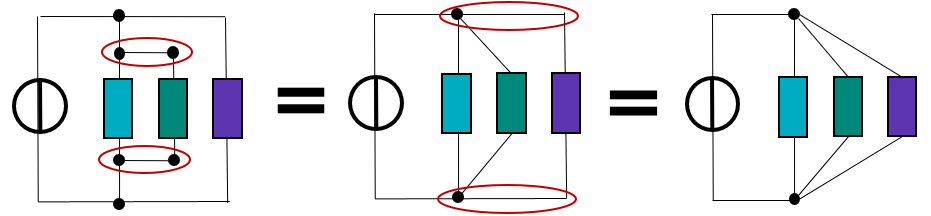
\includegraphics[scale=0.3]{img/knoten-kontrahieren.png}}
						\end{center}
					\iend

					\newpage


					\subsection{Vorgehen um Schaltbilder mit einer Quelle zu vereinfachen}
					\begin{enumerate}
						\item Bringe Quelle auf die linke Seite
						\item Forme mit Regel 1 - 5 das Netzwerk soweit um, bis nur noch Spannungs-/Stromteiler oder einfache Maschen vorhanden sind.
						\item Expandiere nun das Netzwerk Schritt für Schritt, bis die Spannung über dem gesuchten Widerstand berechnet werden kann.
					\end{enumerate}

					\important{Beispiel}{\#1}
					\beginip
					1) Berechnen sie $U_x$ in Abhängigkeit des Quellstromes $I$
					\begin{center}
						\fix
					 \ibox{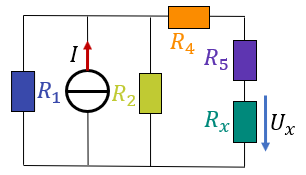
\includegraphics[scale=0.55]{img/aufg1-aufg.png}}
					\end{center}
					\fix
					 \textbf{Lösung}
				 \begin{enumerate}
  				 \item Gemäss Regel 2 können wir $R_1$ und die Stromquelle vertauschen.
					 \item Die Widerstände $R_4 , R_5$ und $ R_x $ können zu $ R_S = R_3 + R_4 + R_5 $ zusammengefasst werden.
					 \item Mithilfe der Stromteilerregel erhalten wir $ I_s = I \cdot \frac{(R_1 || R_2 || R_s)}{R_s} $ und somit $U_s = I \cdot (R_1 || R_2 || R_S) $
					 \item Die Spannung $U_s$ liegt also über dem Widerstand $R_s$ an. Wenn wir diesen wieder in die ursprünglichen 3 Widerstände aufteilen, erhalten wir mithilfe der Spannungsteilerregel $U_x = U_s \cdot \frac{R_x}{R_4 + R_5 + R_x} $
				 \end{enumerate}

					\ibox{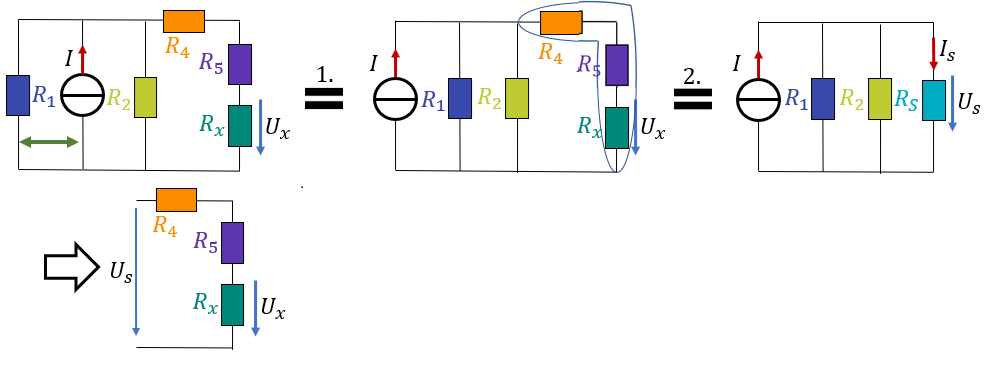
\includegraphics[scale=0.55]{img/bsp1.png}}
					\iend

					In manchen Fällen kann es schwierig sein, die Quelle auf die linke Seite zu bringen oder das Schaltbild nützlich umzuformen. \\
					Um ein erstes Ersatzschaltbild zu erhalten, kann das "Flussverfahren\texttt{"} angewandt werden.

\newpage
					\definition{Flussverfahren}
					\beginip
					Beim Flussverfahren überlegt man sich sämtliche Arten, wie der Strom von einem Ende der Quelle zum anderen fliessen kann, und zeichnet somit ein Ersatzschaltbild. \\ \\
					\textbf{Beispiel}
					\begin{center}
						\fix
							\ibox{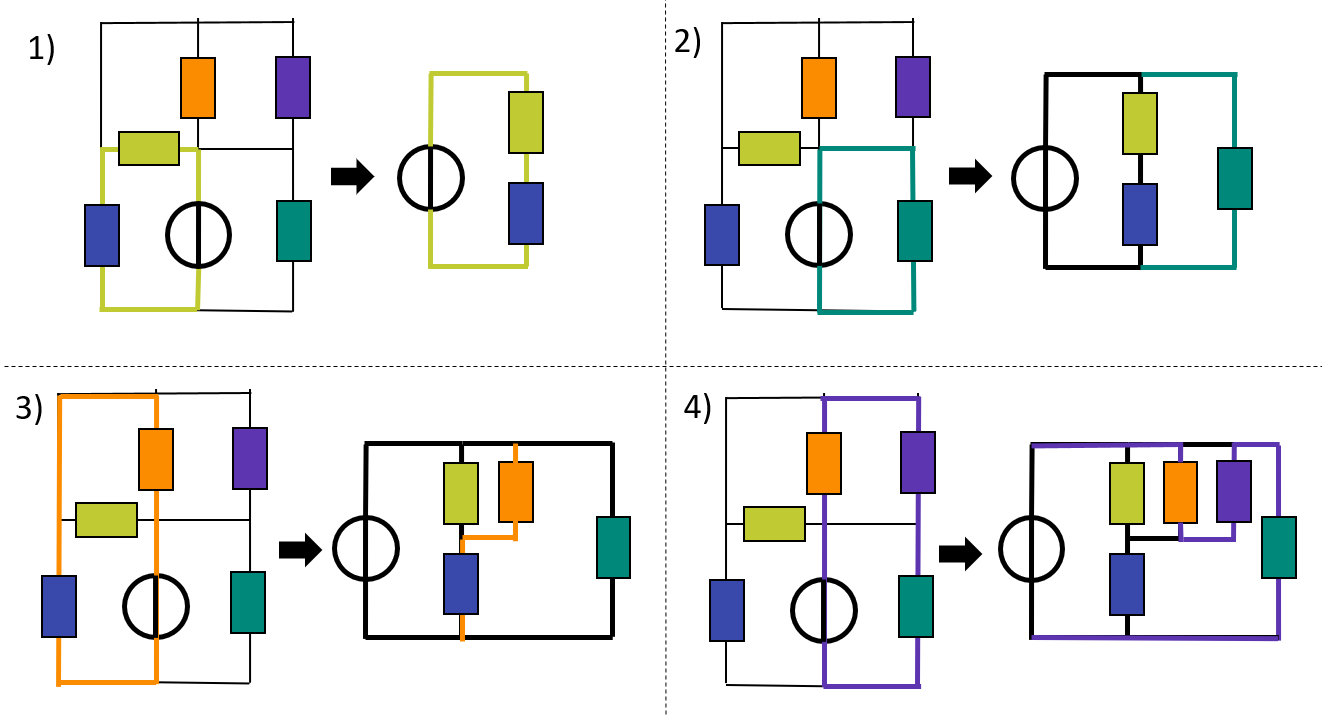
\includegraphics[scale=0.3]{img/fluesse.png}}
					\end{center}
					\iend

					\subsection{Quellen}
					\definition{Ideale Quelle}
					\beginip
					Eine ideale Strom-/Spannungsquelle liefert immer denselben Strom/dieselbe Spannung, unabhängig von der Last, welche angehängt wird.
					\begin{center}
						\ibox{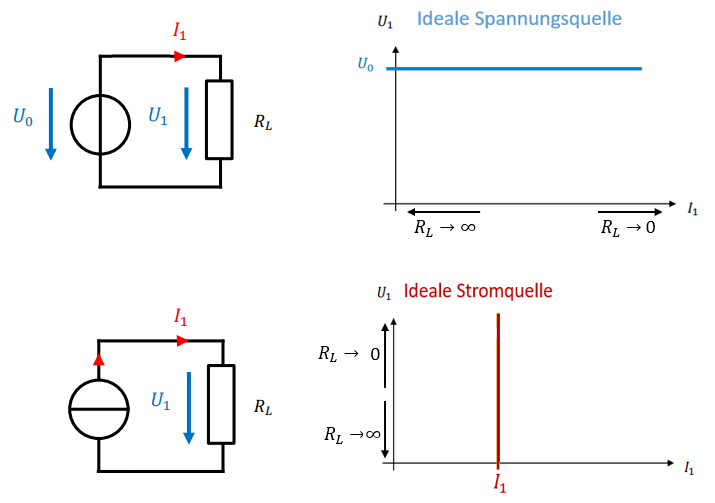
\includegraphics[scale=0.6]{img/ideale_quelle.png}}
					\end{center}

					\iend


					Mit idealen Strom-/Spannungsquellen können wir theoretisch unendlich viel Spannung/Strom über einem Lastwiderstand erzeugen. \\
					(Beispiel ideale Spannungsquelle im Kurzschluss/ideale Stromquelle im Leerlauf) \\
					Bei einer realen Quelle kann jedoch nur eine endliche Spannung/Strom auftreten, wesshalb wir Verluste innerhalb der Quelle mit einem Innenwiderstand $R_i$ modellieren. \\

					\definition{Reale Quelle}
					\beginip
					Eine reale Quelle bezeichnet eine ideale Quelle mit Vorwiderstand. \\
					Bei einer \textbf{Stromquelle} ist der Widerstand \textbf{parallel}, bei einer \textbf{Spannungsquelle} ist der Widerstand in \textbf{Serie}.
						\begin{center}
							\fix
								\ibox{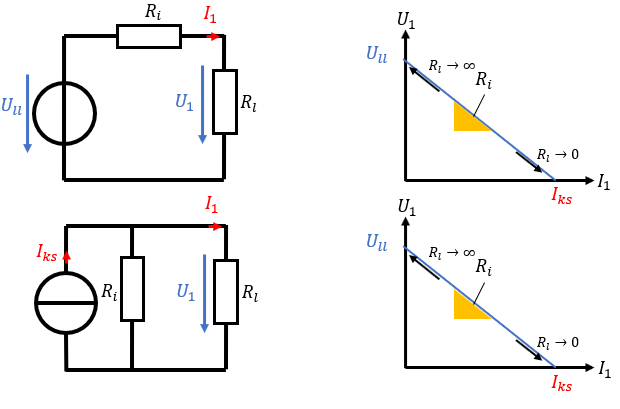
\includegraphics[scale=0.7]{img/realeQuellen.png}}
						\end{center}
					\iend


					\subsection{Leistungsanpassung}
					\definition{Leistung}
					\beginip
						Als Leistung bezeichnen wir das Produkt von Strom und Spannung. \\
						Sie bezeichnet die in einer Zeitspanne umgesetzte Energie an einem Bauteil. \\
						\formulaBegin
						$\displaystyle P := U \cdot I = \frac{U^2}{R} = I^2 \cdot R $
						\formulaEnd
					\iend

					\definition{Maximale Leistung}
					\beginip
					Um bei einer realen Quelle maximale Leistung an einen Lastwiderstand abzugeben, muss der Lastwiderstand gleich gross sein wie der Innenwiderstand der Quelle. \\
					\formulaBegin
					$ R_i = R_L \Rightarrow P = P_{max}$
					\formulaEnd
					\begin{center}
						\ibox{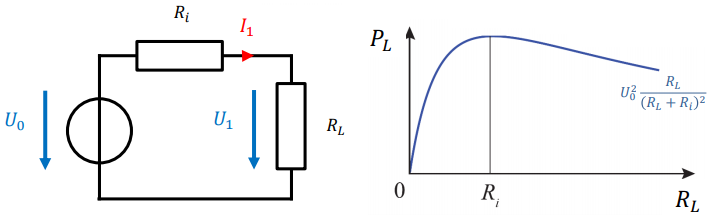
\includegraphics[scale=0.5]{img/leistungsanpassung.png}}
					\end{center}
					\iend

\newpage
					\textbf{Begründung} \\
					Die Leistung an einem Lastwiderstand in Serie ist gegeben als: \\
					$ \displaystyle P_L = U_L \cdot I_L = \frac{U_L^2}{R_L} = \frac{( U_0 \frac{R_L}{R_L + R_i})^2}{R_L} = U_o^2 \cdot \frac{R_L}{(R_L + R_i)^2}$ \\
					$\displaystyle \frac{d}{dR_L} (P_L) = - U_0^2 \cdot \frac{R_L - R_i}{(R + R_L)^3} = 0 \Rightarrow R_L = R_i  \Rightarrow P_L = P_{max}$

					\subsection{Superpositionsprinzip}

					 Das Superpositionsprinzip besagt, dass wir bei einem Netzwerk mit mehreren Quellen einzelne Teillösungen in Abhängigkeit von nur einer Quelle berechnen und aufsummieren können. \\
					 Dies gilt jedoch nicht für die Leistung, da diese nicht linear ist! \\
					 Um das Superpositionsprinzip anzuwenden, müssen wir alle ausser eine Quelle auf \texttt{"}0\texttt{"} setzen. \\
					 Spannungsquellen werden also mit \textbf{Kurzschlüssen} ersetzt und Stromquellen mit \textbf{Leerläufen}. \\
					 \begin{center}
					 	\fix
					 		\ibox{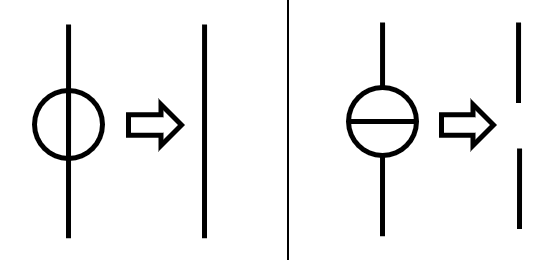
\includegraphics[scale=0.3]{img/superpos-zero.png}}
					 \end{center}


					 \textbf{Wieso} \\
					 Eine Spannungsquelle zu \texttt{"}0\texttt{"} zu setzen bedeutet, dass über diesem Bauteil keine Spannung abfallen darf. Über einem Kurzschluss wird nie eine Spannung abfallen, da dieser als Widerstand mit Wert 0 modelliert werden kann. \\
					 Eine Stromquelle zu \texttt{"}0\texttt{"} zu setzen bedeutet, dass durch dieses Bauteil kein Strom fliessen darf. Dies entspricht gerade einem Leerlauf, da dieser als Widerstand mit Wert $\displaystyle \rightarrow \infty$ modelliert werden kann. \\


					 \important{Beispiel}{\#2}
					 \beginip
						\textbf{Aufgabe} Berechnen sie die Spannung $U_x$ und die Leistung $P_x$ im folgenden Netzwerk, wenn alle Widerstände $ R = 100 \Omega$ betragen. \\
						\begin{center}
							\fix
						\ibox{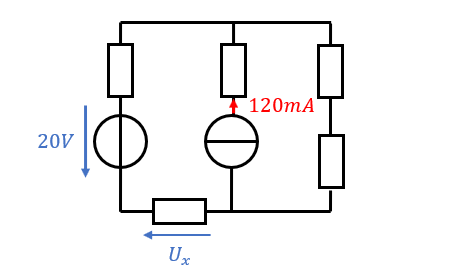
\includegraphics[scale=0.6 ]{img/ex2-1.png}}
						\end{center}
						\iend

						\beginip
						\textbf{Lösung}
						\\
						Zuerst setzen wir die Spannungsquelle zu 0 und erhalten das folgende ESB \\
						\begin{center}
							\fix
						\ibox{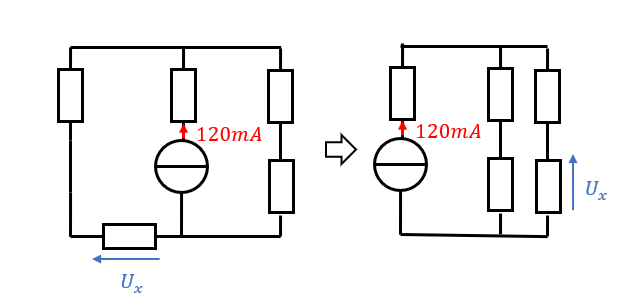
\includegraphics[scale=0.5 ]{img/ex2-2.png}}
						\end{center}

						Nun berechnen wir den Strom $I_{x_1}$ durch den Widerstand mithilfe eines Stromteilers: \\
						$I_{x_1} = 60mA$ \\
						Die Spannung $U_x$ ist entgegen der Stromrichtung eingezeichnet: \\
						$U_{x_1} = - R_x \cdot I_x = - 100 \cdot 60mA = -6V $ \\
						\\
						Nun setzen wir die Stromquelle zu 0: \\
						\begin{center}
							\fix
						\ibox{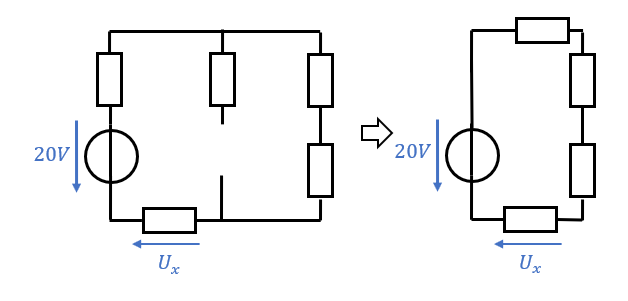
\includegraphics[scale=0.5 ]{img/ex2-3.png}}
						\end{center}

						Die Spannung $U_{x_2}$ berechnet sich als Spannungsteiler: \\
						$U_{x_2} = 20V \cdot \frac{100\Omega}{400\Omega} = 5V$ , $ I_{x_2} = \frac{5V}{100\Omega} = 50mA $\\
						\\
						Schlussendlich berechnet sich die Spannung als Summe der Teilspannungen:
						$U_x = U_{x_1} + U_{x_2} = 5V -6V = -1V $ \\
						Und die Leistung: \\
						$P_x = \frac{{U_x}^2}{R_x} = 10mW$ \\
						Welche \textbf{nicht} der Summe der Teilleistungen entspricht: \\
						$P_{sum} = P_1 + P_2 = U_{x_1} \cdot I_{x_1} + U_{x_2} \cdot I_{x_2} = 360mW + 250mW = 610mW$


					 \iend

					 \newpage
					\definition{Thévenin / Norton Äquivalent}
					\beginip
					Jedes Netzwerk mit \textbf{linearen} Bauelementen und 2 Klemmen lässt sich als reale Quelle darstellen. \\
					\textbf{Thévenin Äquivalent} Darstellung als reale \textbf{Spannungsquelle} mit Leerlaufspannung, die an den Klemmen auftritt \\
					\textbf{Norton Äquivalent} Darstellung als reale \textbf{Stromquelle}  mit Kurzschlussstrom, der an den Klemmen auftritt\\
					Der Innenwiderstand entspricht dem von außen gemessenen Widerstand, wenn alle Quellen zu 0 gesetzt werden.
					\begin{center}
						\fix
							\ibox{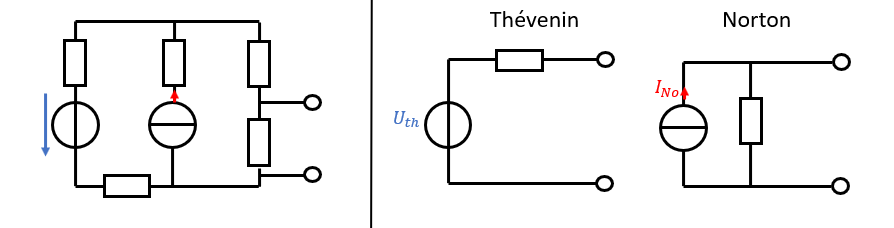
\includegraphics[scale=0.6]{img/nort_the.png}}
					\end{center}
					\iend






					\important{Beispiel}{\#3 - Thévenin Äquivalente Schaltung}
					\beginip
					\textbf{Aufgabe}
					\\Geben sie eine Thévenin Äquivalente Schaltung (Innenwiderstand $R_i$, $U_{Th}$) für folgende Klemmen an. Alle Widerstände haben Wert $100\Omega$ \\

					\begin{center}
						\fix
							\ibox{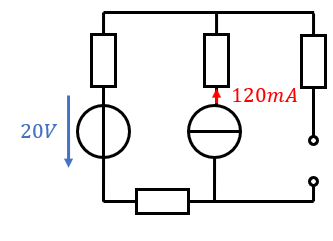
\includegraphics[scale=0.4]{img/ex3-1.png}}
					\end{center}
					\iend
					\beginip
					\textbf{Lösung}
					\\
					Zuerst berechnen wir die Leerlaufspannung für die Stromquelle: \\
					$U_{LL_1} = 120mA \cdot 200 \Omega = 24V$ \\
					Danach die Leerlaufspannung für die Spannungsquelle: \\
					$ U_{LL_2} = 20V$\\
					Die Gesamtspannung und somit die Spannung der Ersatzspannungsquelle beträgt: \\
					$\doubleunderline{U_{Th}} = U_{LL_1} + U_{LL_2} = \doubleunderline{44V}$ \\

					Nun müssen wir noch den Innenwiderstand berechnen. Dazu setzen wir alle Quellen zu 0 und berechnen den von aussen gemessenen Widerstand:\\
					\begin{center}
						\fix
							\ibox{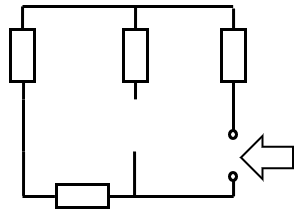
\includegraphics[scale=0.6]{img/ex3-2.png}}
					\end{center}
										$\doubleunderline{R_i} = 100\Omega + 100\Omega  + 100\Omega  = \doubleunderline{300 \Omega} $
					\iend


					\subsection{Maschenstromverfahren}
					Beim Maschenstromverfahren geht es darum, möglichst schnell linear unabhängige Gleichungen zu finden, um alle Grössen im Netzwerk zu berechnen. \\
					Man könnte auch alle Maschen und Knotengleichungen aufstellen und das resultierende Gleichungssystem lösen. \\
					Beide Vorgehen führen zu einem Gleichungssystem, dessen Matrix stets symmetrisch sein muss.
					Durchgerechnete Aufgaben befinden sich auf der Übungswebseite n.ethz.ch/~zrene/elektrotechnik1.html in den Slides für die Übung 5. \\
\newpage

					\important{Vorgehen}{}
					\beginip
					\begin{enumerate}
							\item Mache alle Stromquellen unwirksam (Leerlauf!)
							\item Bestimme nun die reduzierte Menge $E^*$ aller verbleibenden Elementarmaschen
							\item Weise jeder Masche $M_i \in E^*$ einen Maschenstrom $I_i$ zu
							\item Füge die Stromquellen wieder ein und ergänze Maschenströme für die Stromquellen (1 pro Quelle!)
							\item Stelle für jede Masche  $M_i \in E^*$ von Punkt 2 eine Maschengleichung (\textbf{Spannungen!}) auf
							\item Löse das resultierende Gleichungssystem
					\end{enumerate}
					\begin{center}
						\ibox{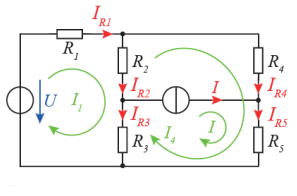
\includegraphics[scale=0.8]{img/maschenstrom.png}}
					\end{center}
					\iend

					\subsection{Knotenpotentialverfahren}
					Auch hier geht es darum, möglichst schnell linear unabhängige Gleichungen zu finden, um alle Grössen im Netzwerk zu berechnen
					\important{Vorgehen}{}
					\beginip
					\begin{enumerate}
						\item  Wähle einen Bezugsknoten $K_0$ (Potential = 0)
						\item Mache alle Spannungsquellen aus (Kurzschluss!)
						\item Weise allen Knoten (ausser $K_0$) ein Potential $\varphi_i$ zu
						\item Füge die Spannungsquellen wieder ein: Dabei werden Knoten aufgetrennt in zwei Knoten, einer bekommt Potential $\varphi_i$, der andere $\varphi_i + U_i$
						\item Stelle für alle Knoten mit unabhängigem Potential eine Knotengleichung auf!
						\item Liegt zwischen zwei Knoten nur eine Spannungsquelle, werden diese als einen einzelnen Knoten betrachtet!

					\end{enumerate}
					\begin{center}
						\ibox{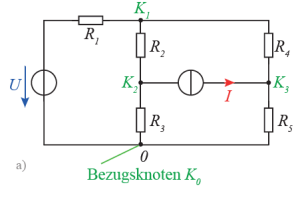
\includegraphics[scale=1]{img/knotenpotential.png}}
					\end{center}
					\iend
